\documentclass[a4paper]{article}
\usepackage[utf8]{inputenc} 
\usepackage[danish]{babel} 

\usepackage{amsmath}
\usepackage{amsfonts}
\usepackage{amssymb}
\usepackage{ulem}
\usepackage{verbatim}
\usepackage{graphicx}
\usepackage{xcolor}
\usepackage{marvosym}

\usepackage{tikz}
\usetikzlibrary{calc,shapes.multipart,chains,arrows}
\tikzset{
squarecross/.style={
    draw, rectangle,minimum size=18pt, fill=orange!80,
    inner sep=0pt, text=black,
    path picture = {
        \draw[black]
        (path picture bounding box.north west) --
        (path picture bounding box.south east)
        (path picture bounding box.south west) --
        (path picture bounding box.north east);
    }
  }
}

\usepackage{listings}
\lstdefinestyle{customc}{
  belowcaptionskip=1\baselineskip,
  breaklines=true,
  frame=L,
  xleftmargin=\parindent,
  language=C,
  showstringspaces=false,
  basicstyle=\footnotesize\ttfamily,
  keywordstyle=\bfseries\color{green!40!black},
  commentstyle=\itshape\color{purple!40!black},
  identifierstyle=\color{blue},
  stringstyle=\color{orange},
}

\lstdefinestyle{customasm}{
  belowcaptionskip=1\baselineskip,
  frame=L,
  xleftmargin=\parindent,
  language=[x86masm]Assembler,
  basicstyle=\footnotesize\ttfamily,
  commentstyle=\itshape\color{purple!40!black},
}

\lstset{escapechar=@,style=customc}

\newcommand*{\mybox}[2]{\colorbox{#1!30}{\parbox{.98\linewidth}{#2}}}
\newcommand{\setR}{\mathbb{R}} 
\newcommand{\setF}{\mathbb{F}} 
\newcommand{\setN}{\mathbb{N}} 
\newcommand{\pder}[2][]{\frac{\partial#1}{\partial#2}}
\newcommand{\RNum}[1]{\uppercase\expandafter{\romannumeral #1\relax}}

\newcommand*{\titleGM}{\begingroup % Create the command for including the title page in the document
	\hbox{ % Horizontal box
		\hspace*{0.2\textwidth} % Whitespace to the left of the title page
		\rule{1pt}{\textheight} % Vertical line
		\hspace*{0.05\textwidth} % Whitespace between the vertical line and title page text
		\parbox[b]{0.75\textwidth}{ % Paragraph box which restricts text to less than the width of the page
			
			{\noindent\Huge\bfseries DMA \\[0.5\baselineskip] }\\[2\baselineskip] % Title
			{\large \textit{Ugeopgave 4}}\\[4\baselineskip] % Tagline or further description
			{\Large \textsc{Beate Berendt Søegaard}}\\ % Author name
			{\Large \textsc{Mathias Larsen}}\\ % Author name
			{\Large \textsc{Simon Rotendahl}} % Author name
			
			\vspace{0.5\textheight} % Whitespace between the title block and the publisher
			{\noindent Datalogi}\\[\baselineskip] \today% Publisher and logo
		}}
		\endgroup}
	
%\title{faget  \\ \Large Aflevering #}
%\author{navn}
\begin{document}
%\maketitle
\titleGM % This command includes the title page
%\tableofcontents
\section*{Del 1}
\subsection*{a}


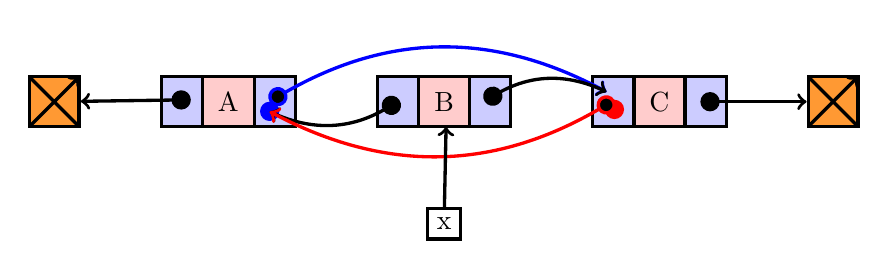
\begin{tikzpicture}[
 list/.style={
        very thick, rectangle split,
        rectangle split parts=3, draw,
        rectangle split horizontal, minimum size=18pt,
        inner sep=5pt, text=black,
        rectangle split part fill={blue!20, red!20, blue!20}
    },
square/.style={rectangle, draw},
    ->, start chain, very thick
  ]

\node[list,on chain] (A) {\nodepart{second} A};
\node[list,on chain] (B) {\nodepart{second} B};
\node[list,on chain] (C) {\nodepart{second} C};
\node[square] (x) [below=of B] {x};

\node[squarecross]   (D) [right=of C] {};
\node[squarecross]   (E) [left= of A] {};

\path[*->] let \p1 = (A.three), \p2 = (A.center) in (\x1,\y2) edge [bend left] ($(C.one)+(0,0.2)$)[draw=blue];
\path[*->] let \p1 = (B.three), \p2 = (B.center) in (\x1,\y2) edge [bend left] ($(C.one)+(0,0.2)$);
\draw[*->] let \p1 = (C.three), \p2 = (C.center) in (\x1,\y2) -- (D);

\draw[*->] ($(A.one)+(0.2,0.1)$) -- (E);
\path[*->] ($(B.one)+(0.1,0.1)$) edge [bend left] ($(A.three)+(0,-0.05)$);
\path[*->] ($(C.one)+(0.1,0.1)$) edge [bend left] ($(A.three)+(0,-0.05)$)[draw=red];
\draw[->] (x) -- ($(B.two)+(0.15,-0.2)$);
\end{tikzpicture}\\
Da listen skal være dobbelthægtet skal en knude have tre felter. En previous, en key, ($x$'et) og en next felt. 

\subsection*{b}

\begin{lstlisting}
(1) n = doubly-link list
(2) z = n.key
(3) x = S.head
(4)  fun F(S,z)
(5)  if z.key <= S.head then 
(6) 	 z.next = S.head.next
(7) 	 z = S.head
(8) 	 z.prev = NULL
(9)  elif z.key => S.tail 
(10)	 z.next = NULL
(11)	 S.tail.next = z
(12) 	 z.prev = S.tail
(13)     S.tail = z
(14) else 
(15) 	 z.next = x.next 
(16)     z.prev = x
(17)     x.next = z
(18) while z.key > x.key and x.next != NULL
(19)     x = x.next
\end{lstlisting}

\subsection*{c}
I vores pseudokode har vi tre samlignings statements, hvilket køre i $\mathcal{O}(1)$. Tilsidst har vi et \text{while-løkke} som køre i $\mathcal{O}(n)$ tid. Dvs., at køretiden for pseudokoden er $T(n) = \mathcal{O}(1)+\mathcal{O}(1)+\mathcal{O}(1)+\mathcal{O}(n) = \mathcal{O}(n)$.\\
Udover det så da vi har flere nestede operatorer, f.eks linje 10 til linje 13 er nestede i linje 9. Det vil sige at køretiden for linje 10 - 13 skal summeres og derefter ganges på linje 9's kørertid. Det betyder dog ikke noget for vores køretid da alle nestede operationer er af konstanttid, og derved ikke øger den samlede størrelsesorden. 
\subsection*{d}
\textit{Lad listen S være tom til at starte med. Der indsættes herefter $n$ heltal. Et af gangen. Når det sidste heltal er indsat vil S være en sorteret liste bestående af	de $n$ indsatte tal. Argumentér for at vi på denne måde har sorteret $n$ tal i $\mathcal{O}(n^2)$ tid.}

Køretiden for vores funktion kan deles op i to dele: Søge og indsættelse. Vi starter med at analysere indsættelse 

\textbf{Søge:} Antallet af operationer for $n$, vil være summen af antallet af $n-1$ heltal (det skal være $n-1$ da det element der indsættes ikke skal sammenlignes med sig selv). F.eks hvis der er $n = 4$ heltal der skal sættes ind i S, så vil summen være $0+1+2+3=6$ så 6 operationer er nødvendige. Antallet af operationer der er nødvendige for en given mængde heltal $n$, vil være lig med $$\frac{n\times(n-1)}{2}$$ hvilket kan findes i CLRS side 1146 (dog går den sumfunktion til $n$ og ikke $n$-1, derfor er vores ændret). Vi kan se fra regel S6 omkring størrelsesorden at $\frac{n\times(n+1)}{2}$ har samme størrelsesorden som $\frac{n\times(n+1)}{2}\times2$ og derved kan vi fjerne konstanterne fra udtrykket, og derefter ganger vi parantesen ud, og får $n^2 + n^1$. Med regel S3 kan vi vise at $n^1$ er af lavere størrelsesorden end $n^2$ og med regel S8 kan vi vise at en funktion af lavere størrelsesorden adderet med en funktion af højere størrelsesorden, vil have samme størrelsesorden som den høje funktion. Derved har vi vist at $$\frac{n\times(n+1)}{2}\times2 \in \Theta(n^2)$$ 

\textbf{Indsættelse:} Det tager dog også $n$ tid at indsætte elementerne i S, og derved vil den samlede søge og indsættelses funktions størrelsesorden lyde $$n^2+n$$ Vi har dog lige vist at + $n$ ikke betyder noget for størrelsesordnen og derved ikke køretiden, så endeligt bliver køretiden $\mathcal{O}(n^2)$
\newpage
\section*{Del 2}
\subsection*{a}
En liste $S$ kan opdeles i $k$ mindre sorterede lister, $l_1, l_2, \cdots l_k$, hvor hver af de $k$ små lister, består af $k$ elementer. Vi får endvidere oplyst at $k=\sqrt n$ er et heltal, dvs. at hver $l_k$ skal være lige store.
Knuderene i $B$ bliver oprettet ved $k=\sqrt n$.

\subsection*{b}
Da $B$ består af $k$ elementer tager det $\mathcal{O}(k)$ tid at løbe igennem det. 
$k$ er defineret som $k = \sqrt{n}$, hvor n er antallet af elementer i $S$ så derfor 
kan vi også skrive tiden det tager at løbe $B$ igennem som $\mathcal{O}(\sqrt{n})$.

\subsection*{c}
\lstset{language=python} 
\begin{lstlisting} 
(1) G(S, B, x)
(2)  i = B.head
(3)  if i.pa > x then
(4)      x.prev = NIL
(5)      x.next = S.head
(6)      i.pa.prev = x
(7)      S.head = x
(8)   loop until i == NIL 
(9)       if i.next.pa > x OR i.next == NIL then
(10)         I = i.pa
(11)         loop until I == i.next.pa OR I == NIL
(12)            if I >= x then
(13)                x.next = I
(14)                x.prev = I.prev
(15)                I.prev.next = x
(16)                I.prev = x
(17)                return S
(18)            I = I.next        
\end{lstlisting}   

\end{document}